\section{برنامه ریزی برای مقایس های طولی مختلف}
در عمل ، ممکن است که یه نمایش نقشه و الگوریتم برنامه ریزی کافی نباشد. برای مثال برای برنامه
 ریزی مسیر یک خودرو ممکن است یه جستوجوی ناهنجار روی شبکه خیابان انجام بشه مانند عملیات در
 سیستم مسیریاب ماشین ، ولی برنامه ریزی راجب اینکه کدوم راه باید انتخاب بشه دخیل نیست.

برنامه ریزی راه ها و اینکه چطوری دوربرگردان ها و تقاطع ها مسیر یابی بشوند، می بایست لایه از برنامه
 ریزی گسسته داشته باشد. اینکه چطوری ربات را حرکت بدیم در یک مسیر و از موانع اجتناب کنیم  با 
الگوریتم های های
\rl{sampling-based} 
مناسب تر است. مسیر ها برنامه ریزی شده احتیاج دارند که در
 نهایت به سرعت چرخ و زاویه چرخش ها با استفاده از کنترل های بازخورد تبدیل شوند. این مراتب در
 شکل
\ref{fig:scale}
  نمایش داده شده. 
 \begin{figure}[H]
  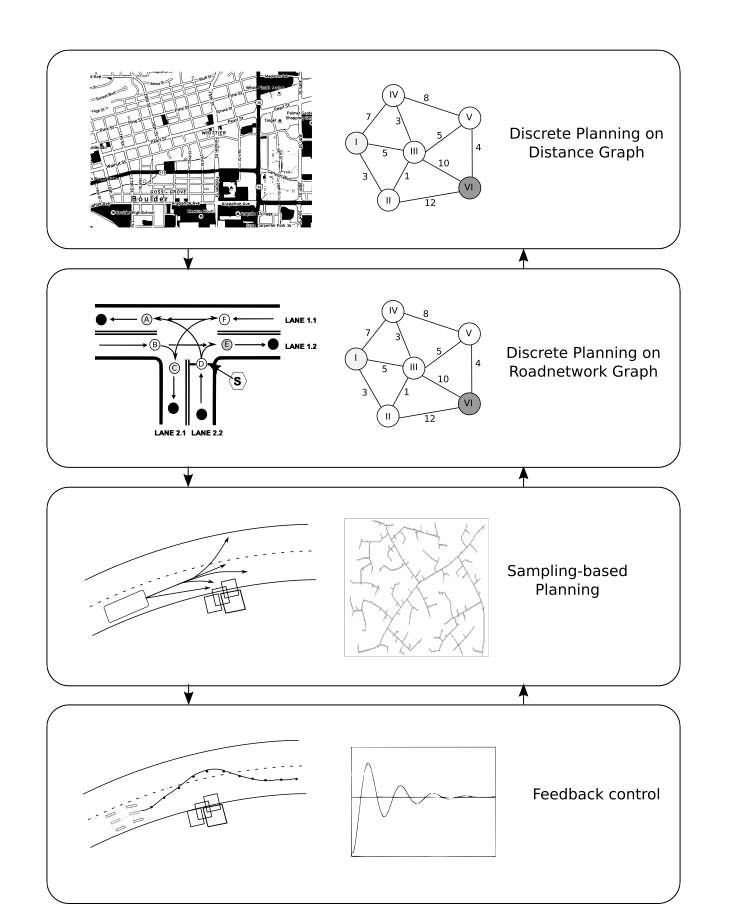
\includegraphics[width = \textwidth]{images/scale.png}
  \caption{برنامه ریزی مسیر در مقیاس های طولی مختلف}
  \label{fig:scale}
\end{figure}
\par
در اینجا این آرایه های جهت پایین ورودی های است که لایه بالایی برنامه ریزی برای لایه ی پایینی را فراهم
 میکند، نشون می دهد. و نشانگر های جهت بالا، است‍‍ثنا هایی که با لایه مرحله پایین تر قابل بیان نیست را
 نشان میدهند. برای مثال یک کنترل کننده ی بازخورد نمیتواند موانع رو پوشش دهد و به یک برنامه ریزی
\rl{sampling-based} 
  نیاز داریم. 
یک وضعیت مشابه برای هدایت ربات ها می توان درست کرد که به چندین نوع از نمایش و کنترل کننده برای برنامه و انجام مسیریابی به صورت بهینه نیاز دارد.
توجه کنید که در این نمایش  سطح استدلالی که قانون  راهنمایی و رانندگی و قضاوت درست را کدگذاری کند استفاده نمی شود. ولی ممکن است یک سری از این، با استفاده از توابع هزینه مانند بیشترین مسافت از موانع یا اطمینان از رانندگی روان و ثابت یا رفتار های پیچیده تر مثل سازگار کردن رانندگی در صورت حضور سرنشین یا ویژگی های سطح زمین که به لایه های بیشتر عمودی نیاز دارد(که به همه لایه برنامه ریزی دسترسی دارد) پیاده سازی شود.

